\documentclass{beamer}
\usepackage{sdp}

\title{Редици}

\date{16 октомври 2015 г.}

\titlegraphic{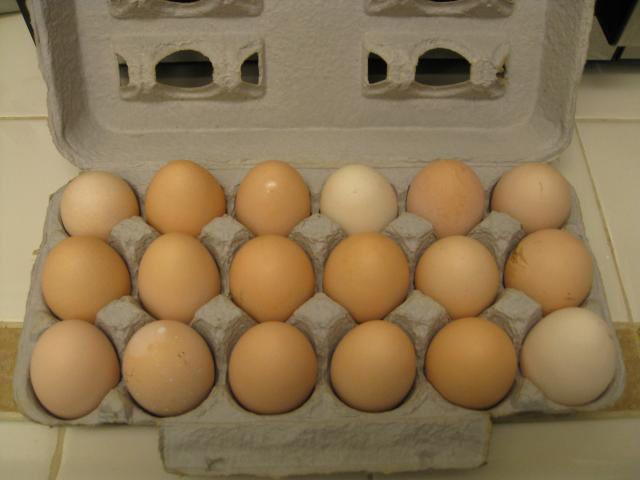
\includegraphics[height=0.3\textheight]{images/array.jpg}}

\begin{document}

\begin{frame}
  \titlepage
\end{frame}

\section{Масиви}

\begin{frame}
  \frametitle{АТД: Масив}

  Последователност от елементи от еднакъв вид, които могат да бъдат избирани по номер (индекс).
  \vspace{1em}

  Операции
  \begin{itemize}
  \item \tt{create(n)} --- създаване на масив със зададена големина
  \item \tt{get(i)} --- получаване на елемент с индекс \tt i
  \item \tt{set(i,x)} --- задаване на стойност \tt x на елемента с индекс \tt i
  \item \tt{size} --- дължина на масива 
  \end{itemize}
  \vspace{1em}

  Свойства на операциите
  \begin{itemize}
  \item \tt{a.set(i,x).get(i)} = \tt x
  \item \tt{a.set(i,x).get(j)} = \tt{a.get(j)}, ако \tt{i $\neq$ j}
  \item \tt{create(n).size} = \tt n
  \end{itemize}
\end{frame}

\begin{frame}
  \frametitle{Статично представяне}

  \begin{tabular}{|c|c|c|c|c|c|c|c|}
    \rowcolor{blue!60!green!40}
    \hline
    $a_0$&$a_1$&$a_2$&\ldots&\ldots&\ldots&\ldots&$a_{n-1}$\\
    \hline
    \multicolumn{8}{c}{$\underbrace{\hspace{40ex}}_{\text{дължина}}$}\\
  \end{tabular}
  \vspace{3em}

  Реализация: масив във C++.

  \tt{int a[10];}

\end{frame}

\begin{frame}
  \frametitle{Динамично представяне}
  \newcommand{\pha}{\hspace{2ex}}

  \begin{tabular}{|c|c|c|c|c|c|c|c|c|c|c|c|c|c|c|c|}
    \multicolumn{16}{c}{$\overbrace{\hspace{60ex}}^{\text{капацитет}}$}\\
    \rowcolor{blue!60!green!40}
    \hline
    $a_0$&$a_1$&$a_2$&\ldots&\ldots&\ldots&\ldots&$a_{n-1}$&\pha&\pha&\pha&\pha&\pha&\pha&\pha&\pha\\
    \hline
    \multicolumn{8}{c}{$\underbrace{\hspace{40ex}}_{\text{дължина}}$}\\
  \end{tabular}
  \vspace{3em}

  Реализация: \tt{std::vector}.

\end{frame}

\begin{frame}
  \frametitle{\tt{std::vector<T>}}

  Реализация на динамичен масив
  \begin{itemize}
  \item \tt{vector(n)} --- създава вектор с дължина \tt n
  \item \tt{size} --- дължина на вектора
  \item \tt{capacity} --- капацитет на вектора
  \item \tt{[i]}, \tt{at(i)} --- достъп до елемент на индекс \tt i
  \item \tt{front()}, \tt{back()} --- достъп до първи и последен елемент
  \item \tt{push\_back(x)} --- добавяне на елемента \tt x в края
  \item \tt{pop\_back()} --- изтриване на последния елемент
  \item \tt{insert(...)} --- вмъкване на елементи на произволна позиция
  \item \tt{erase(...)} --- изтриване на елементи на произволна позиция
  \end{itemize}
\end{frame}

\begin{frame}
  \frametitle{\tt{std::string}}
\end{frame}

\section{Кортежи}

\begin{frame}
  \frametitle{АТД: Наредена двойка}

  Двойка от елементи от потенциално различен тип, в която редът има значение.

  Операции
  \begin{itemize}
  \item \tt{create(a,b)} --- създава двойка от елементите \tt a и \tt b
  \item \tt{p.first} --- връща първия елемент на двойката
  \item \tt{p.second} --- връща втория елемент на двойката
  \end{itemize}

  Свойства на операциите
  \begin{itemize}
  \item \tt{create(a,b).first} = \tt a
  \item \tt{create(a,b).second} = \tt b
  \item \tt{create(p.first,p.second)} = \tt p
  \end{itemize}
\end{frame}

\begin{frame}[fragile]
  \frametitle{Физическо представяне}

  \begin{center}
    \begin{tabular}{|m{3ex}|m{5ex}|}
      \hline
      \rowcolor{blue!60!green!40}
      \centering a&\centering b\\
      \hline
    \end{tabular}
  \end{center}
  \vspace{2em}

  Реализации:
  \begin{itemize}
  \item \verb#struct Pair{ int first; char second; };#
  \item \verb#std::pair<T,U>#
  \end{itemize}
\end{frame}

\begin{frame}
  \frametitle{\tt{std::pair}}
\end{frame}

\begin{frame}
  \frametitle{АТД: Кортеж}
\end{frame}

\end{document}
